\documentclass[a4paper]{article}
\usepackage{amsfonts}
\usepackage{amsmath}
\usepackage{amssymb}
\usepackage{graphicx}     

\begin{document}
  
\noindent \large Auteur: Stan Van Campenhout \\
\noindent \large Studierichting:  Informatica\\
\noindent \large Oefeningenreeks 3H nr. 8.7\\

\medskip

\normalsize

$ r = 2\cos6\theta $\\

$ \operatorname{dom} = \mathbb{R} $\\

$ p = \dfrac{\pi}{3} $\\

$ \rightarrow \operatorname{BD} = [0 , \dfrac{\pi}{3}] $\\

$ r = 0 \Leftrightarrow 2\cos6\theta = 0 \Leftrightarrow6\theta = \dfrac{\pi}{2} + k\pi \Leftrightarrow \theta =  \dfrac{\pi}{12} +  k\dfrac{\pi}{6},  \forall k \in \mathbb{Z} $\\

$ \rightarrow \left\{\dfrac{\pi}{12}, \dfrac{\pi}{4}\right\} $\\

$ r' = 0 \Leftrightarrow -2\sin6\theta = 0 \Leftrightarrow 6\theta =k\pi \Leftrightarrow \theta = k\dfrac{\pi}{6},  \forall k \in \mathbb{Z} $\\

$ \rightarrow \left\{0, \dfrac{\pi}{6}, \dfrac{\pi}{3}\right\} $\\

\begin{tabular}{ l | c c c c c c c c r }	
  $\theta$ &$0$ & &$\dfrac{\pi}{12}$ & &$\dfrac{\pi}{6}$ & &$\dfrac{\pi}{4}$ & &$\dfrac{\pi}{3}$\\ \hline
  $r$ &$+$ &$+$ &$0$ &$-$ &$-$ &$-$ &$0$ &$+$ &$+$\\
  $r'$ &$0$ &$-$ &$-$ &$-$ &$0$ &$+$ &$+$ &$+$ &$0$\\ \hline
  $r$ &$M$ &$\nearrow$ &$\nearrow$ &$\nearrow$ &$m$ &$\searrow$ &$\searrow$ &$\searrow$ &$M$\\
    &$2$ & & & &$-2$ & & & &$2$\\
\end{tabular}

\begin{figure}[h]
\centering
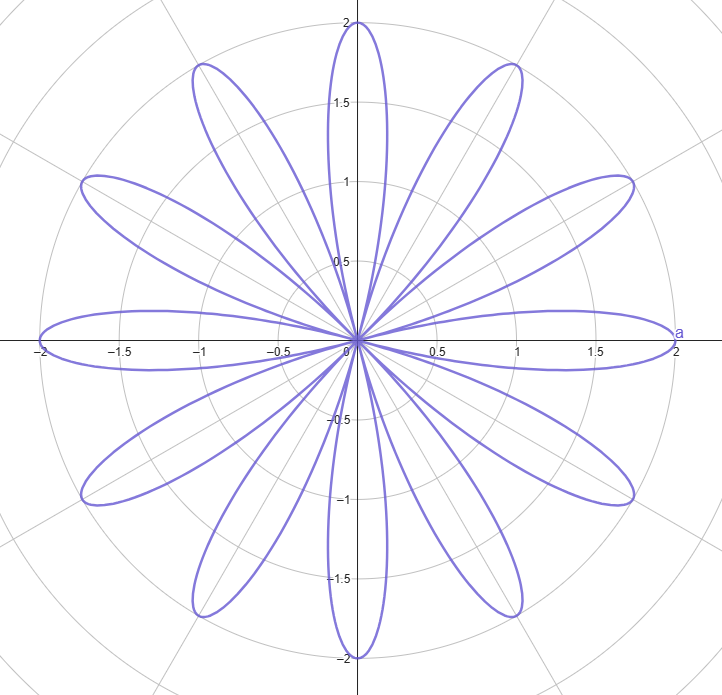
\includegraphics[width=7cm]{3H-8.7-stan.van.campenhout.INF.png}
\end{figure}

\begin{thebibliography}{999}
%\bibitem{a} Referentie
\end{thebibliography}
\end{document} 
